\documentclass{ctexart}
\usepackage{graphicx}
\usepackage{geometry}
\usepackage{amsmath}
\usepackage{color}
\usepackage[colorlinks,linkcolor = black]{hyperref}
\usepackage{listings}
\geometry{left = 3cm,right = 3cm,top = 2.5cm, right = 2.5cm}

\definecolor{mygreen}{rgb}{0,0.6,0}
\definecolor{mygray}{rgb}{0.5,0.5,0.5}
\definecolor{mymauve}{rgb}{0.58,0,0.82}
\lstset{ %
	backgroundcolor=\color{white},   % choose the background color
	basicstyle=\ttfamily,        % size of fonts used for the code
	columns=fullflexible,
	breaklines=true,                 % automatic line breaking only at whitespace
	captionpos=b,                    % sets the caption-position to bottom
	tabsize=4,
	commentstyle=\color{mygreen},    % comment style
	escapeinside={\%*}{*)},          % if you want to add LaTeX within your code
	keywordstyle=\color{blue},       % keyword style
	stringstyle=\color{mymauve}\ttfamily,     % string literal style
	frame=single,
	% rulesepcolor=\color{red!20!green!20!blue!20},
	% identifierstyle=\color{red},
	% language=c++,
}

\begin{document}
		\title{CS229 Machine Learning Problem Set 1}
		\author{Wang Minhu}
		\date{9, Sep, 2017}
		\maketitle
		\clearpage
	\section{Logistic Regression}
	\subsection{1}
	
	考虑仅有一个样本点的情况, 此时
	
	\begin{equation}
		J(\theta) = log(1 + e^{-y\theta^Tx})
	\end{equation}
	
	考虑
	
	\begin{align}
		\frac{\partial J(\theta)}{\partial \theta_i \theta_j} &= \frac{\partial}{\partial \theta_i}(\frac{-e^{-y\theta^Tx}}{1 + e^{-y\theta^Tx}} x_j y) \notag \\
		&= \frac{e^{-\theta^Txy}(1 + e^{-\theta^Txy}) - (e^{-\theta^Txy})^2}{(1 + e^{-y\theta^Tx})^2}x_i x_j y^2 \notag \\
		&= \frac{e^{-\theta^Txy}}{(1 + e^{-y\theta^Tx})^2}x_i x_j y^2
	\end{align}
	
	对任意矢量$z$, 有
	
	\begin{align}
		z^THz &= \sum_i \sum_j H_{ij} z_i z_j = \sum_i \sum_j \frac{e^{-\theta^Txy}}{(1 + e^{-y\theta^Tx})^2} y^2 x_i x_j z_i z_j \notag \\
		&= \frac{e^{-\theta^Txy}}{(1 + e^{-y\theta^Tx})^2} y^2 \sum_i \sum_j  x_i x_j z_i z_j \notag \\
		&= \frac{e^{-\theta^Txy}}{(1 + e^{-y\theta^Tx})^2} y^2 (x^Tz)^2 \ge 0
	\end{align}
	这一结论很容易扩展到多个样本点, 记
	\begin{align}
		J_i(\theta) = log(1 + e^{-y^{(i)}\theta^Tx^{(i)}})
	\end{align}
	则有
	\begin{align}
		J(\theta) &= \frac{1}{m}\sum_i^m J_i(\theta) \\
		H &= \frac{1}{m} \sum_i^m H_i
	\end{align}
	因此
	
	\begin{equation}
		z^THz = \frac{1}{m}\sum_i^m z^TH_iz \ge 0 
	\end{equation}
	
	因此这是一个半正定矩阵.
	
	\subsection{2}
	
	Newton方法的迭代公式为
	\begin{equation}
		\theta = \theta - H^{-1} \nabla_{\theta}l(\theta)
	\end{equation}
	
	此处
	\begin{align}
		\nabla_{\theta}l(\theta) &= \frac{1}{m}\sum_{i=1}^m \frac{y^{(i)}}{1 + e^{y^{(i)}\theta^Tx^{(i)}}}x^{(i)} \\
		H &=  \frac{1}{m}\sum_{i=1}^m\frac{e^{-\theta^Tx^{(i)}y^{(i)}}y^{(i)2}}{(1 + e^{-y^{(i)}\theta^Tx^{(i)}})^2}x^{(i)}x^{(i)T} 
	\end{align}
	
	写出MATLAB代码
	
	\begin{lstlisting}[language = MATLAB]
% Function to calculate the cost in logistic regression
%   INPUT: variable x in training set, variable y in training set,
%   parameters theta
%   OUTPUT: cost

function loss = cost(x, y, theta)
	m = size(x,1);
	loss = sum(-log(sigmoid(x, y, theta))) / m;
end

% Function to calculate the derivative vector of the cost function for
% introducing Newton's method
%   INPUT: variable x[m * n_x] in training set, variable y[m * 1] in training set,
%   parameters theta[n*x * 1]
%   OUTPUT: derivative vector [n_x * 1]

function d = derivative(x, y, theta)
	m = size(x,1);
	d = -sum((y .* sigmoid(x, -y, theta)) .* x)/m;
end

% Function to calculate the hessian matrix of the cost function for
% introducing Newton's method
%   INPUT: variable x[m * n_x] in training set, variable y[m * 1] in training set,
%   parameters theta[n*x * 1]
%   OUTPUT: hessian matrix h[n_x * n_x]

function [ h ] = hessian( x, y, theta )
	s = sigmoid(x, y, theta);
	m = (size(x, 1));
	h = (x' * (((s .* (1 - s)) .* (y .^ 2)) .* x)) ./ m;
end

% Function to get value of the sigmoid function as part of calculations
% of the cost/derivate/hessian
%   INPUT: variable x[m * n_x] in training set, variable y[m * 1] in training set,
%   parameters theta[n*x * 1]
%   OUTPUT: sigmoid function value s[m * 1]

function s = sigmoid(x,y,theta)
	s = 1 ./ (1 + exp(-y .* (x * theta)));
end

% load the training set and initialize the parameters and cost list vector
train_x = load("assets/logistic_x.txt");
train_y = load("assets/logistic_y.txt");
train_x(:,size(train_x,2) + 1) = ones(size(train_x,1),1);
theta = zeros(size(train_x,2),1);
lostlist = zeros(1,500);

% apply the Newton's method to train the logistic regression model
for i = 1:500

	lostlist(1,i) = cost(train_x, train_y, theta);
	d = derivative(train_x, train_y , theta);
	h = hessian(train_x, train_y, theta);
	theta = theta - h\(d');    

end
	\end{lstlisting}
	
最终得到的参数为\verb|[0.760;1.172;-2.621]|

\subsection{3}
实际上
\begin{equation}
	h_\theta(x) > 0.5 \to \frac{1}{1 + e^{-\theta^Tx}} > 0.5 \to \theta^Tx > 0 \notag
\end{equation}
因此在图中画出$\theta^Tx = 0$线即可.

\begin{lstlisting}[language = MATLAB]
% draw the distribution of training data and the final model
ind1 = train_y == 1;
ind2 = train_y == -1;
scatter(train_x(ind1,1), train_x(ind1,2),'g');
hold on;
scatter(train_x(ind2,1), train_x(ind2,2),'r');
hold on;
x = 0:8;
y = -(theta(1) * x + theta(3))/theta(2);
plot(x,y);
\end{lstlisting}
得到图\ref{logistic}.

\begin{figure}[ht]
	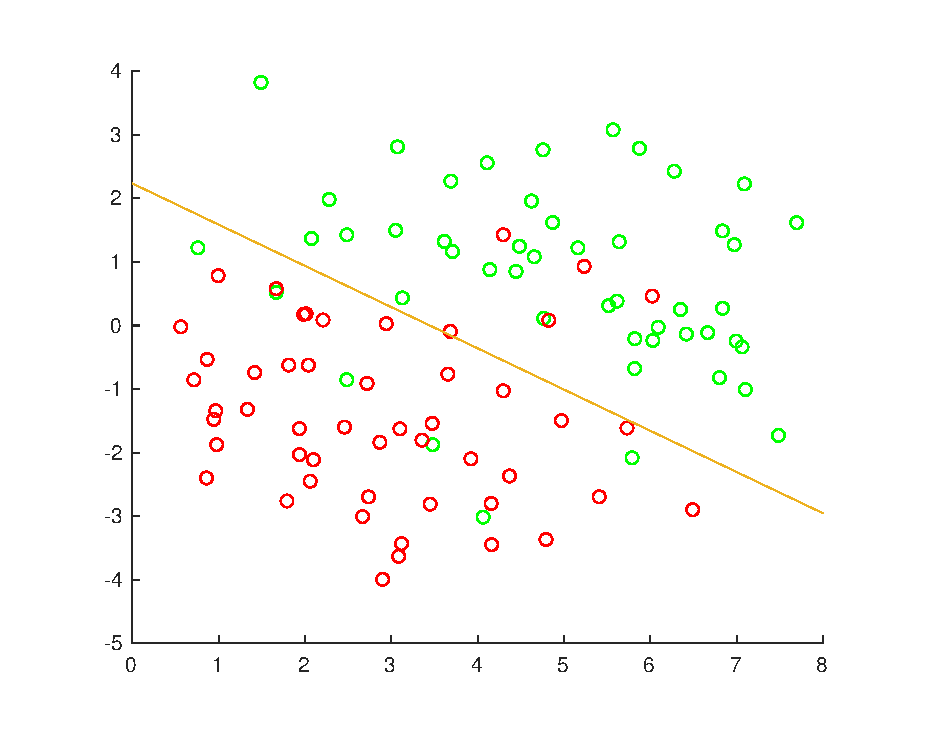
\includegraphics[width = \textwidth]{logistic.eps}
	\caption{logistic回归及其训练集}
	\label{logistic}
\end{figure}

\section{Possion Regression}
\subsection{1}

对Possion分布的概率密度稍作变换
\begin{align}
	p(y;\lambda) = \frac{e^{-\lambda}\lambda^y}{y!} = \frac{e^{ylog\lambda-\lambda}}{y!}
\end{align}

通过比较系数可得

\begin{align}
	b(y) &= \frac{1}{y!} \notag \\
	\eta &= \log(\lambda) \notag \\
	T(y) &= y \notag \\
	a(\eta) &= \lambda = e^{\eta}  \notag
\end{align}

因此Possion分布属于指数分布族.

\subsection{2} 
\begin{equation*}
	h_\theta(x) = E[y|x;\theta] = \lambda = e^\eta = e^{\theta^T x}
\end{equation*}

\subsection{3}

假设只有一个样本点
\begin{equation}
	l(\theta) = \log(L(\theta)) = \log(\frac{e^{-\lambda}\lambda^y}{y!}) = -\lambda + y \log(\lambda) - \log(y!)
\end{equation}

则有
\begin{equation}
	\frac{\partial l(\theta)}{\partial \theta_j} = -e^{\theta^Tx}x_j + yx_j = (y - e^{\theta^Tx})x_j
\end{equation}

因此随机梯度下降的学习规则是

\begin{equation}
	\theta_j:= \theta_j + \alpha(y^{(i)} - e^{\theta^Tx^{(i)}})x_j^{(i)}
\end{equation}

\subsection{4}
我们有下式恒成立

\begin{equation}
	\int_{-\infty}^{\infty} b(y)e^{\eta y - a(\eta)}dy =e^{-a(\eta)} \int_{-\infty}^{\infty} b(y)e^{\eta y}dy =1
\end{equation}

两边对$\eta$求导

\begin{equation}
	-e^{-a(\eta)}\frac{\partial a(\eta)}{\partial \eta} \int_{-\infty}^{\infty} b(y)e^{\eta y}dy + e^{-a(\eta)} \int_{-\infty}^{\infty} yb(y)e^{\eta y}dy = 0 \notag
\end{equation}

整理得到

\begin{equation}
-\frac{\partial a(\eta)}{\partial \eta} \int_{-\infty}^{\infty} b(y)e^{\eta y - a(\eta)}dy +  \int_{-\infty}^{\infty} yb(y)e^{\eta y - a(\eta)}dy = E(y;\eta) - \frac{\partial a(\eta)}{\partial \eta} = 0 \notag
\end{equation}

因此有

\begin{equation}
	E(y;\eta) = \frac{\partial a(\eta)}{\partial \eta}
\end{equation}

考虑单样本情况, 其最大似然对数

\begin{equation}
	l(\theta) = \log(p(y;\eta)) = \log(b(y)) + \eta y - a(\eta) \notag
\end{equation}

计算其导数

\begin{equation}
\frac{\partial l(\theta)}{\partial \theta_j} = yx_j - \frac{\partial a(\eta)}{\partial \eta} \frac{\partial \eta}{\partial \theta_j} = (y - E(y;\eta))x_j = (y-h_\theta(x))x_j
\end{equation}

因此对于任意$T(y) = y$的GLM, 其随机梯度下降的学习规则皆为
\begin{equation}
\theta_j:= \theta_j + \alpha(y^{(i)} - e^{\theta^Tx^{(i)}})x_j^{(i)}
\end{equation}

\section{Gaussian Discriminant Analysis}

\subsection{1}

\begin{align}
	p(y = 1|x) &= \frac{p(x|y = 1)P(y = 1)}{p(x|y = 1)P(y = 1) + p(x|y = 0)P(y = 0)} \notag \\
	&=  \frac{p(x|y = 1)\phi}{p(x|y = 1)\phi + p(x|y = 0)(1 - \phi)} \notag \\
	&=  \frac{\phi}{\phi + \frac{p(x|y = 0)}{p(x|y = 1)}(1 - \phi)} \notag \\
	&=  \frac{\phi}{\phi + e^{\frac{1}{2}[(x-\mu_1)^T\Sigma^{-1}(x-\mu_1)-(x-\mu_{-1})^T\Sigma^{-1}(x-\mu_{-1})]}(1 - \phi)} \notag \\
	&= \frac{\phi}{\phi + e^{\frac{1}{2}[u_{-1}^T\Sigma^{-1}-u_1^T\Sigma^{-1} + u_{-1}^T \Sigma^{-1} - u_1 \Sigma^{-1}]x + \frac{1}{2}[u_1^T\Sigma^{-1}u_1 - u_{-1}^T\Sigma^{-1}u_{-1}]}(1 - \phi)} \notag \\
	&= \frac{1}{1 + e^{[u_{-1}^T\Sigma^{-1}-u_1^T\Sigma^{-1}]x + \frac{1}{2}[u_1^T\Sigma^{-1}u_1 - u_{-1}^T\Sigma^{-1}u_{-1}]}(\frac{1}{\phi} - 1)} \notag \\
\end{align}

对比系数可得
\begin{align}
	\theta^T &= -(u_{-1}^T\Sigma^{-1}-u_1^T\Sigma^{-1}) \\
	\theta_0 &= -\frac{1}{2}(u_1^T\Sigma^{-1}u_1 - u_{-1}^T\Sigma^{-1}u_{-1}) + \log(\frac{1}{\phi} - 1)
\end{align}

\subsection{2}

当$n=1$时, 概率退化为

\begin{align}
	p(x|y= -1) = \frac{1}{(2\pi)^{\frac{1}{2}}\sigma}e^{-\frac{(x-\mu_{-1})^2}{2\sigma^2}} \\
	p(x|y= -1) = \frac{1}{(2\pi)^{\frac{1}{2}}\sigma}e^{-\frac{(x-\mu_{1})^2}{2\sigma^2}}	
\end{align}

首先讨论$\phi$

\begin{align}
	l(\phi,\mu_{-1},\mu_1,\Sigma) &= \log(\prod_{i=1}^m p(x^{(i)}|y^{(i)};\mu_{-1},\mu_1,\Sigma)p(y^{(i)};\phi)) \notag \\
	&= \log(\prod_{i=1}^m p(x^{(i)}|y^{(i)};\mu_{-1},\mu_1,\Sigma)) + \log(\prod_{i=1}^m(p(y^{(i)};\phi)) \notag \\
\end{align}

记
\begin{align*}
M = \sum_{i=1}^m 1\{y^{(i)} = 1\} \\
N = \sum_{i=1}^m 1\{y^{(i)} = -1\} \\	
\end{align*}

对$\phi$求导

\begin{align}
	\frac{\partial l}{\partial \phi} &= \frac{\partial \log(\prod_{i=1}^m(p(y^{(i)};\phi))}{\partial \phi} \notag \\
	&= \frac{\partial \sum_{i=1}^m \log(p(y^{(i)};\phi))}{\partial \phi} \notag \\
	&= \frac{\partial(Mlog(\phi) + N\log(1-\phi))}{\partial \phi} \notag \\
	&= \frac{M}{\phi} - \frac{N}{1-\phi} = 0 \notag
\end{align}

解出

\begin{equation}
	\phi = \frac{M}{M+N}  =\frac{1}{m}  \sum_{i=1}^m 1\{y^{(i)} = 1\}
\end{equation}

注意这一结论不依赖于n的阶数.

讨论$\mu_1$

\begin{align*}
		\frac{\partial l}{\partial \mu_1} &= \frac{\partial \log(\prod_{i=1}^m p(x^{(i)}|y^{(i)};\mu_{-1},\mu_1,\Sigma))}{\partial \mu_1} \notag \\
		&=  \frac{\partial \sum_{i=1}^m\log( p(x^{(i)}|y^{(i)};\mu_{-1},\mu_1,\Sigma))}{\partial \mu_1} \notag \\
		&=  \frac{\partial \sum_{i=1}^m\log(\frac{1}{(2\pi)^{\frac{1}{2}}\sigma}e^{-\frac{(x^{(i)}-\mu_{y^{(i)}})^2}{2\sigma^2}})}{\partial \mu_1} \notag \\
		&=  \frac{-\partial \sum_{i=1}^m \frac{(x^{(i)} - \mu_{y^{(i)}})^2}{2 \sigma^2}}{\partial \mu_1} \notag \\
		&= \sum_{i = 1}^m 1\{y^{(i)} = 1\}\frac{x^{(i)} - \mu_1}{\sigma^2} = 0
\end{align*}

整理得

\begin{equation}
	\mu_{1} = \frac{\sum_{i=1}^m 1\{y^{(i)} = 1\} x^{(i)}}{\sum_{i=1}^m 1\{y^{(i)} = 1\}}
\end{equation}

由$\mu_1$和$\mu_{-1}$的对称性, 可以直接写出

\begin{equation}
\mu_{-1} = \frac{\sum_{i=1}^m 1\{y^{(i)} = -1\} x^{(i)}}{\sum_{i=1}^m 1\{y^{(i)} = -1\}}
\end{equation}

讨论$\Sigma$
\begin{align*}
\frac{\partial l}{\partial \sigma} &= \frac{\partial \log(\prod_{i=1}^m p(x^{(i)}|y^{(i)};\mu_{-1},\mu_1,\Sigma))}{\partial \Sigma} \notag \\
&=  \frac{\partial \sum_{i=1}^m\log( p(x^{(i)}|y^{(i)};\mu_{-1},\mu_1,\Sigma))}{\partial \Sigma} \notag \\
&=  \frac{\partial \sum_{i=1}^m\log(\frac{1}{(2\pi)^{\frac{1}{2}}\Sigma}e^{-\frac{(x^{(i)}-\mu_{y^{(i)}})^2}{2\sigma^2}})}{\partial \Sigma} \notag \\
&=  \frac{ \partial (-m\log((2\pi)^{\frac{1}{2}}\sigma) -\sum_{i=1}^m \frac{(x^{(i)} - \mu_{y^{(i)}})^2}{2 \sigma^2})}{\partial \Sigma} \notag \\
&= (-\frac{m}{\sigma} + \sum_{i=1}^m\frac{(x^{(i)} -\mu_{y^{(i)}})^2}{\sigma^3})\frac{d \sigma}{d \Sigma} = 0
\end{align*}

整理得

\begin{equation}
	\Sigma = \sigma^2 = \frac{\sum_{i=1}^m(x^{(i)} - \mu_{y^{(i)}})^2}{m}
\end{equation}

\subsection{3}

注意上述关于$\phi$的讨论并不依赖$n$的阶数, 因而
\begin{equation}
\phi = \frac{1}{m} \sum_{i=1}^m 1\{y^{(i)} = 1\}
\end{equation}

而

\begin{align*}
\frac{\partial l}{\partial \mu_1} &= \frac{\partial \log(\prod_{i=1}^m p(x^{(i)}|y^{(i)};\mu_{-1},\mu_1,\Sigma))}{\partial \mu_1} \notag \\
&=  \frac{\partial \sum_{i=1}^m\log( p(x^{(i)}|y^{(i)};\mu_{-1},\mu_1,\Sigma))}{\partial \mu_1} \notag \\
&=  \frac{\partial \sum_{i=1}^m\log(\frac{1}{(2\pi)^{\frac{n}{2}}|\Sigma|^{1/2}}e^{-\frac{1}{2}(x^{(i)}-\mu_{y^{(i)}})^T |\Sigma|^{-1} (x^{(i)}-\mu_{y^{(i)}})})}{\partial \mu_1} \notag \\
&=  \frac{\frac{1}{2}\partial \sum_{i=1}^m (x^{(i)}-\mu_{y^{(i)}})^T |\Sigma|^{-1} (x^{(i)}-\mu_{y^{(i)}})}{\partial \mu_1} \notag \\
&= \frac{1}{2}\sum_{i=1}^m 1\{y^{(i)} = 1\}(|\Sigma|^{-1} + (|\Sigma|^{-1})^T)(x^{(i)} - \mu_{y^{(i)}}) = 0
\end{align*}

最后一个等式使用了式
\begin{equation*}
\frac{\partial X^TAX}{\partial X} = (A + A^T)X
\end{equation*}

整理得

\begin{equation}
 	\mu_{1} = \frac{\sum_{i=1}^m 1\{y^{(i)} = 1\} x^{(i)}}{\sum_{i=1}^m 1\{y^{(i)} = 1\}}
\end{equation}

类似的可以得到

\begin{equation}
\mu_{-1} = \frac{\sum_{i=1}^m 1\{y^{(i)} = -1\} x^{(i)}}{\sum_{i=-1}^m 1\{y^{(i)} = 1\}}
\end{equation}

关于$\Sigma$
\begin{align*}
\frac{\partial l}{\partial \sigma} &= \frac{\partial \log(\prod_{i=1}^m p(x^{(i)}|y^{(i)};\mu_{-1},\mu_1,\Sigma))}{\partial \Sigma} \notag \\
&=  \frac{\partial \sum_{i=1}^m\log( p(x^{(i)}|y^{(i)};\mu_{-1},\mu_1,\Sigma))}{\partial \Sigma} \notag \\
&=  \frac{\partial \sum_{i=1}^m\log(\frac{1}{(2\pi)^{\frac{n}{2}}|\Sigma|^{(1/2)}}e^{-\frac{1}{2}(x^{(i)}-\mu_{y^{(i)}})^T |\Sigma|^{-1} (x^{(i)}-\mu_{y^{(i)}})})}{\partial \Sigma} \notag \\
&=  \frac{ \partial (-m\log((2\pi)^{\frac{n}{2}}|\Sigma|^{(1/2)}) -\sum_{i=1}^m -\frac{1}{2}(x^{(i)}-\mu_{y^{(i)}})^T |\Sigma|^{-1} (x^{(i)}-\mu_{y^{(i)}}))}{\partial \Sigma} \notag \\
&= (-\frac{m}{2|\Sigma|} + \frac{1}{2}\sum_{i=1}^m\frac{(x^{(i)} -\mu_{y^{(i)}})(x^{(i)} -\mu_{y^{(i)}})^T}{|\Sigma|^2})\frac{\partial |\Sigma|}{\partial \Sigma} = 0
\end{align*}

最后一个等式使用了式
\begin{equation*}
	\frac{\partial X^TAX}{\partial A} = XX^T
\end{equation*}

整理得到
\begin{equation}
\Sigma = \frac{\sum_{i=1}^m(x^{(i)} - \mu_{y^{(i)}})(x^{(i)} - \mu_{y^{(i)}})^T}{m}
\end{equation}

\section{Linear invariance of optimization algorithm}

\subsection{1}

$x^{(i)}$的更新规则

\begin{equation}
	x^{(i+1)} = x^{(i)} - H_f^{-1} \nabla_x f(x) \notag
\end{equation}

$z^{(i)}$ 的更新规则
\begin{equation}
	z^{(i+1)} = z^{(i)} - H_g^{-1} \nabla_z g(z)	\notag
\end{equation}

\begin{equation}
	\frac{\partial g(z)}{\partial z} = \frac{\partial f(Az)}{\partial z} = \frac{\partial Az}{\partial z} \frac{\partial f(Az)}{\partial Az} = A^T \nabla_x f(x)
\end{equation}

\begin{equation}
	H_g = \frac{\partial}{\partial z}(\frac{\partial g(z)}{\partial z})^T = A^T \frac{\partial}{\partial Az}(A^T \frac{\partial f(Az)}{\partial Az})^T = A^T H_f A
\end{equation}

由此得到
\begin{equation}
	z^{(i+1)} = z^{(i)} - A^{-1}H_f^{-1}(A^T)^{-1}A^T\nabla_xf(x) = A^{-1}(x^{(i)} - H_f^{-1}\nabla_xf(x)) = A^{-1}x^{(i+1)}
\end{equation}

通过初始条件$z^{0} = A^{-1} x^{(0)}$, 利用数学归纳法可以导出结论.

\subsection{2}
$x^{(i)}$的更新规则

\begin{equation}
x^{(i+1)} = x^{(i)} -  \nabla_x f(x) \notag
\end{equation}

$z^{(i)}$ 的更新规则
\begin{equation}
z^{(i+1)} = z^{(i)} - \nabla_z g(z) = z^{(i)} - A^T\nabla_x f(x) = A^{-1}(x^{(i)} - AA^T\nabla_x f(x))	\ne A^{-1}x^{(i+1)}\notag
\end{equation}

因此梯度下降法不是重参数化不变的.

\section{Regression for Denoising Quasar Spectra}
\subsection{}
\subsubsection{}
\begin{equation}
	J(\theta) = \frac{1}{2} \sum_{i=1}^{m} \omega^{(i)}(\theta^T x^{(i)} - y^{(i)})^2 = (X\theta - y)^T W(X\theta -y) \notag
\end{equation}

\begin{equation}
	W = \begin{bmatrix}
	w^{1} & 0 & \cdots & 0 \\
	0 & w^{2} & \cdots & 0 \\
	\cdots& \cdots &\cdots & \cdots \\
	0 & 0 & \cdots & w^{m}
	\end{bmatrix}
\end{equation}

\subsubsection{}

\begin{equation}
	\frac{\partial J(\theta)}{\partial \theta} = \frac{\partial (X\theta - y)}{\partial \theta} \frac{\partial J(\theta)}{\partial (X\theta - y)} = 2X^TW(X\theta - y) = 0
\end{equation}

由此得到

\begin{equation}
	X^TWX\theta = X^TWy
\end{equation}

\subsubsection{}
最大化其最大似然的对数
\begin{align}
	l(\theta) &= \log L(\theta) = \log(\prod_{i=1}^m \frac{1}{\sqrt{2\pi}\sigma^{(i)}}e^{-\frac{(y^{(i)}-\theta^T(x^{(i)})^2}{2(\sigma^{(i)})^2}})  \notag \\
	&= -\sum_{i=1}^m\log(\sqrt{2\pi}\sigma^{(i)}) - \sum_{i=1}^m \frac{(y^{(i)}-\theta^T(x^{(i)})^2}{2(\sigma^{(i)})^2} \notag \\
\end{align}

最大化$l(\theta)$, 即最小化

$$
	\sum_{i=1}^m \frac{(y^{(i)}-\theta^T(x^{(i)})^2}{2(\sigma^{(i)})^2}
$$

即解加权系数为
$$
	w^{(i)} = \frac{1}{(\sigma^{(i)})^2}
$$

的加权线性回归.

\subsection{2}

\subsubsection{1}
\begin{lstlisting}[language = MATLAB]
d = quasar_train(2,:);
% construct x 
x = [lambdas, ones(size(lambdas,1),1)];
y = d';
% use nornal equation to get theta instead of the gradient descent method
theta = (x' * x) \ x' * y;
scatter(lambdas, d', 20, 'g');
hold on;
plot(lambdas, theta(1) * lambdas + theta(2));	
\end{lstlisting}

\begin{figure}[ht]
	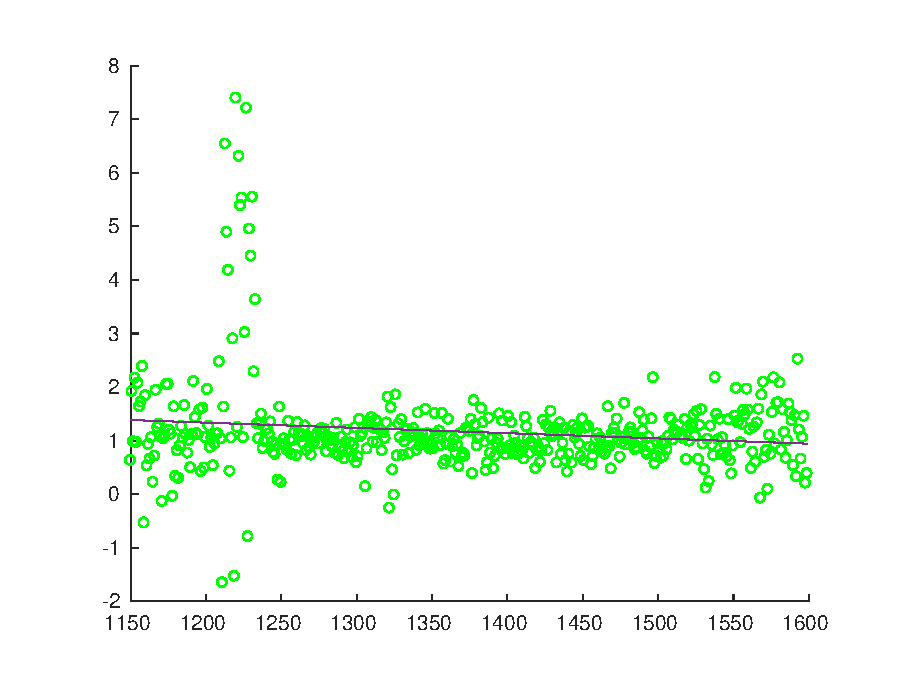
\includegraphics[width = \textwidth]{linear_regression.eps}
	\caption{linear regression}
	\label{logistic}
\end{figure}

\subsubsection{2}

\begin{lstlisting}[language = MATLAB]
d = quasar_train(2,:);
% construct x 
x = [lambdas, ones(size(lambdas,1),1)];
y = d';
% use nornal equation to get theta instead of the gradient descent method
tau = [1,5,10,100,1000];
y_predict = zeros(size(lambdas,1),5);
for k = 1:size(tau,2)
	for i = 1:size(lambdas, 1)
		W = diag(exp(-((lambdas(i,1) - x(:,1)') .^ 2) ./ (2 * (tau(1,k) ^ 2))));
		theta = (x' * W * x) \ (x' * W * y);
		y_predict(i,k) = theta(1) * lambdas(i,1) + theta(2);
	end
	plot(lambdas, y_predict(:,k));
	hold on;
end
scatter(lambdas, d', 20, 'b');
legend('tau = 1','tau = 5', 'tau = 10', 'tau = 100', 'tau = 1000', 'train data');
hold on;
\end{lstlisting}

\begin{figure}[ht]
	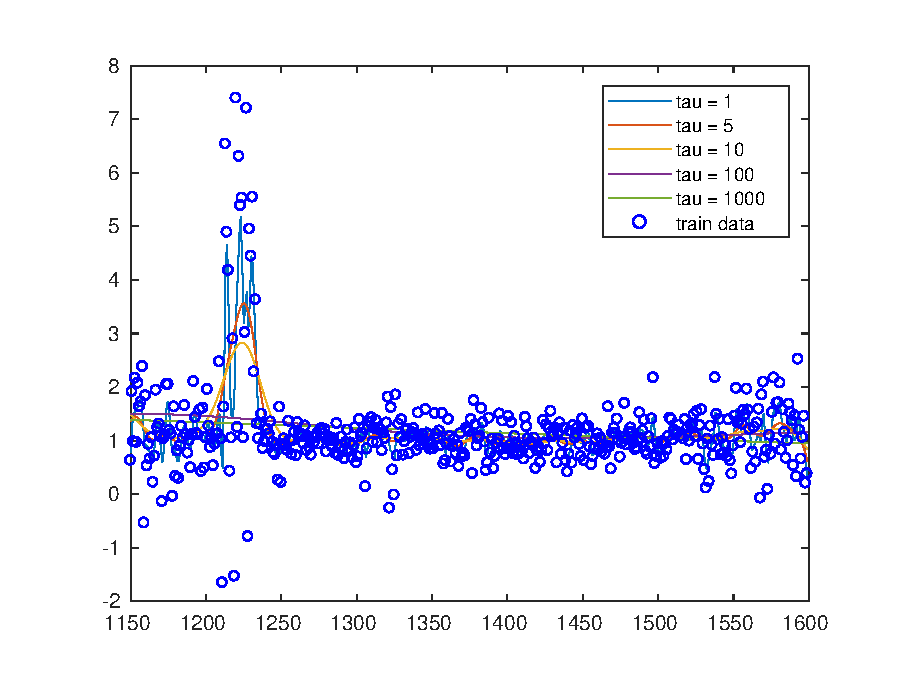
\includegraphics[width = \textwidth]{weight_linear_regression.eps}
	\caption{加权线性回归}
	\label{logistic}
\end{figure}

$\tau$值越大, 加权线性回归对于局部值越不敏感, 越接近于正常的回归, 当$\tau$值比较小时, 回归曲线的波动比较大, 受单值影响很大.

\section{3}

按照说明写出MATLAB程序

\begin{lstlisting}[language = MATLAB]
% function to smooth training and test data with locally weighted
% regressions
% INPUT: 
% data[m * n], m is the number of the training data, n is the length
% of a training sample
% lambdas[n * 1], lambdas is the corresponding wavelength of the data of
% intensity
% 
% OUTPUT:
% smooth_data[m * n], data smoothed with locally weighted regressions

function smooth_data = smooth(data, lambdas)
	% use nornal equation to get theta instead of the gradient descent method
	x = [lambdas, ones(size(lambdas,1),1)];
	tau = 5;
	smooth_data = zeros(size(data,1),size(data,2));
	
	for k = 1:size(data, 1)
		y = data(k,:)';
		for i = 1:size(data,2) 
			W = diag(exp(-((lambdas(i,1) - x(:,1)') .^ 2) ./ (2 * (tau ^ 2))));
			theta = (x' * W * x) \ (x' * W * y);
			smooth_data(k,i) = theta(1) * lambdas(i,1) + theta(2);
		end
	end
end

% Function to calculate the distance defined in the problem of the right
% part of two spectra
% INPUT:
% spectra f1,f2 [1 * n], n is the length of wavelength vector
% OUTPUT:
% distance d, scalar

function d = distance(f1, f2)
	d = sum((f1(151:end) - f2(151:end)) .^ 2);
end

% Function to calculate the distance defined in the problem of the left
% part of two spectra
% INPUT:
% spectra f1,f2 [1 * n], n is the length of wavelength vector or the length
% of left part prediction vector
% OUTPUT:
% distance d, scalar

function d = distance_left(f1, f2)
	d = sum((f1(1:50) - f2(1:50)) .^ 2);
end

% Function to calculate the denotation ker
% INPUT:
% t, scalar
% OUTPUT:
% k, max{1-t, 0}
function k = ker(t)
	k = max(1-t,0);
end

% smooth the data
smooth_train_qso = smooth(train_qso, lambdas);
smooth_test_qso = smooth(test_qso, lambdas);
% set neighbor = 3
k = 3;

f_left_errors = 0;

% use the training data set to test the functional regression
for j = 1:size(smooth_train_qso,1)
	f_right = smooth_train_qso(j,:);
	
	% calculate the distance between f_right with each f^(i)_right in the
	% training set
	dis_list = zeros(size(smooth_train_qso,1),1);
	for i = 1:size(smooth_train_qso,1)
		dis_list(i,1) = distance(smooth_train_qso(i,:), f_right);
	end
	
	[V I] = sort(dis_list);
	
	den = zeros(1,50);
	num = 0;
	for i = 1:k
		den = den + ker(V(i)/V(end)) * smooth_train_qso(I(i),1:50);
		num = num + ker(V(i)/V(end));
	end
	
	f_left = den/num;
	f_left_errors = f_left_errors + distance_left(f_left, smooth_train_qso(j,:));
end

ave_f_left_error = f_left_errors / size(smooth_train_qso,1);

f_left_errors_t = 0;

% use the training test set to test the functional regression
for j = 1:size(smooth_test_qso,1)
	f_right = smooth_test_qso(j,:);
	
	dis_list = zeros(size(smooth_train_qso,1),1);
	for i = 1:size(smooth_train_qso,1)
		dis_list(i,1) = distance(smooth_train_qso(i,:), f_right);
	end
	
	[V I] = sort(dis_list);
	
	den = zeros(1,50);
	num = 0;
	for i = 1:k
		den = den + ker(V(i)/V(end)) * smooth_train_qso(I(i),1:50);
		num = num + ker(V(i)/V(end));
	end
	
	f_left = den/num;
	f_left_errors_t = f_left_errors_t + distance_left(f_left, smooth_test_qso(j,:));
	
	if(j == 1)
		plot(lambdas, smooth_test_qso(j,:)');
		hold on;
		plot(lambdas(1:50), f_left');
	end
end

ave_f_left_error_t = f_left_errors_t / size(smooth_test_qso,1);
\end{lstlisting}

在训练集上取得的平均误差为$1.0664$, 在测试集上取得的平均误差为$2.7100$.

\begin{figure}[ht]
	\parbox{.5\textwidth}{
		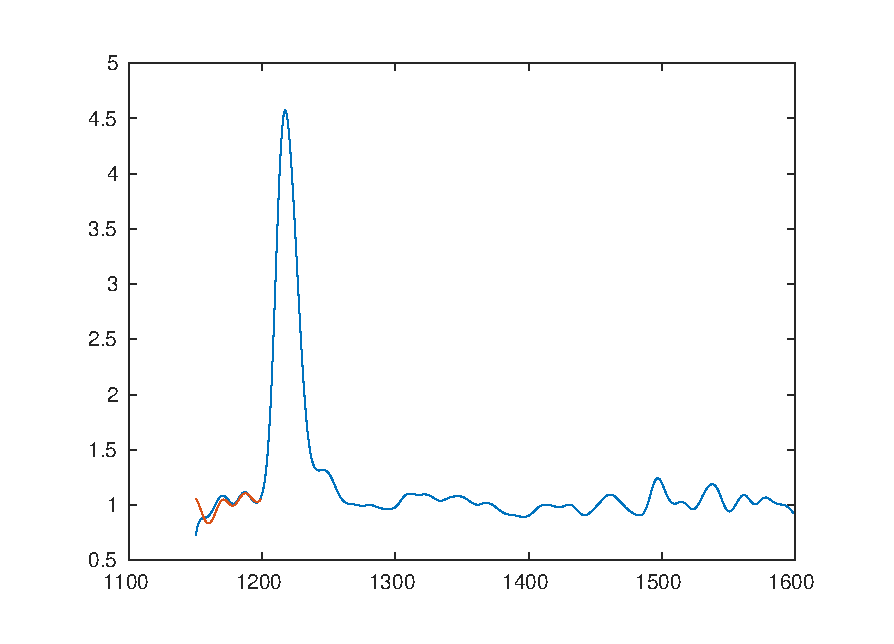
\includegraphics[width = .5\textwidth]{functional_regression_example1.eps}
		\caption{测试集合1-拟合}
		\label{logistic}
	}
	\parbox{.5\textwidth}{
		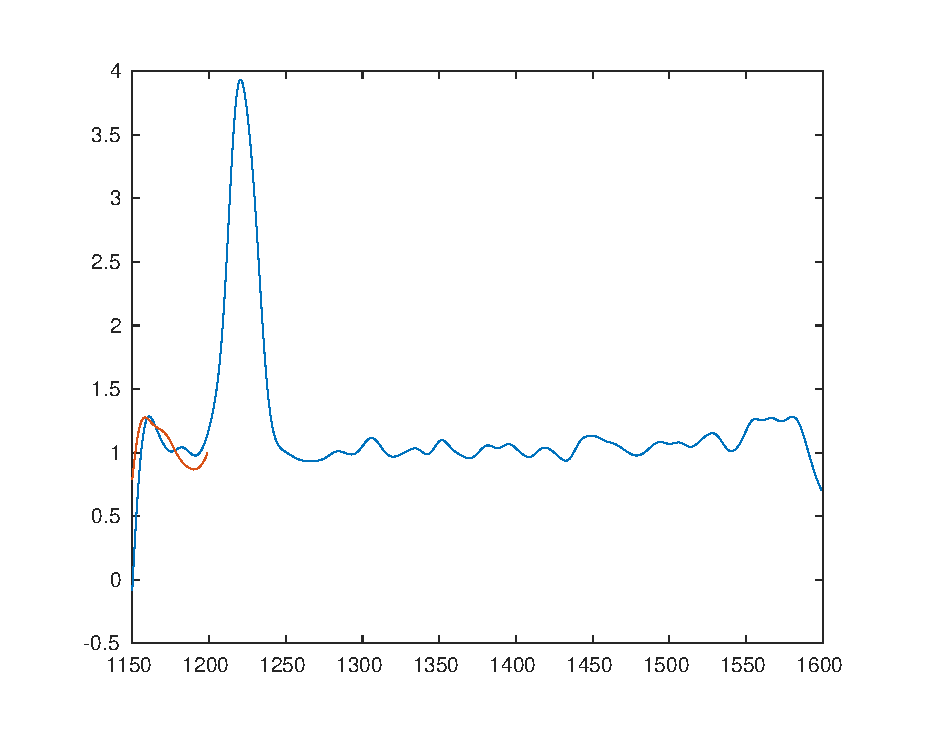
\includegraphics[width = .5\textwidth]{functional_regression_example6.eps}
		\caption{测试集合6-拟合}
		\label{logistic}
	}
\end{figure}

\end{document}